%%
%% This is file `yanputhesis-sample.tex',
%% generated with the docstrip utility.
%%
%% The original source files were:
%%
%% yanputhesis.dtx  (with options: `sample')
%% Copyright (C) 2022 by Shangkun Shen
%%
%% It may be distributed and/or modified under the conditions of the LaTeX
%% Project Public License, either version 1.3b of this license or (at your
%% option) any later version. The latest version of this license is in
%%     https://www.latex-project.org/lppl.txt
%% and version 1.3b or later is part of all distributions of LaTeX version
%% 2005/12/01 or later.
%%=============================================================================%
%% 设置论文格式(学位、盲评、Adobe 字体)
%%-----------------------------------------------------------------------------%
\documentclass[lang=chs, degree=phd, blindreview=false, adobe=true]{yanputhesis}
%%=============================================================================%
%% 导言区:请自行添加额外宏包
%%-----------------------------------------------------------------------------%
\usepackage{blindtext}                                      % 生成无意义文本
\usepackage{metalogo}                                       % 软件标志
\usepackage[binary-units=true]{siunitx}                     % 物理量单位
\usepackage{amsmath}                                        % 基础数学库
%%=============================================================================%
%% 参考文献(也可以是独立文件)
%%-----------------------------------------------------------------------------%
\begin{filecontents}{reference.bib}
@software{NWPUThesisLaTeXTemplate,
  title     = {Yet Another {{\LaTeX}} Template for NPU Thesis},
  author    = {Shangkun Shen and Zhihe Wang and Jiduo Zhang and Weijia Zhang},
  month     = {11},
  year      = {2019},
  publisher = {Zenodo},
  journal   = {GitHub repository},
  doi       = {10.5281/zenodo.4159248},
  url       = {https://doi.org/10.5281/zenodo.4159248}
}

@book{knuth1986the,
  title     = {The {{\TeX}}book},
  author    = {Knuth, Donald E},
  publisher = {Addison-Wesley},
  year      = {1986}
}

@book{lamport1989latex,
  title     = {{{\LaTeX}}: a document preparation system},
  author    = {Lamport, Leslie},
  publisher = {Addison-Wesley Professional},
  year      = {1989}
}

@article{szegedy2015going,
  title   = {Going deeper with convolutions},
  author  = {Szegedy, Christian and Liu, Wei and Jia, Yangqing and
             Sermanet, Pierre and Reed, Scott E and Anguelov, Dragomir and
             Erhan, Dumitru and Vanhoucke, Vincent and Rabinovich, Andrew},
  journal = {Computer Vision and Pattern Recognition},
  pages   = {1--9},
  year    = {2015}
}

@software{MathSymbolsinLaTeXbypolossk,
  title     = {Math Symbols in {{\LaTeX}}},
  author    = {Shangkun Shen},
  year      = {2017},
  month     = {10},
  publisher = {Zenodo},
  journal   = {GitHub repository},
  doi       = {10.5281/zenodo.4120375},
  url       = {https://doi.org/10.5281/zenodo.4120375}
}

@article{chen2014maiyuan,
  title   = {脉源三支 强强融合——西北工业大学},
  author  = {{陈家忠}},
  journal = {电子技术与软件工程},
  number  = {9},
  pages   = {15--16},
  year    = {2014}
}

@article{shen2021peridynamic,
  title     = {Peridynamic modeling with energy-based surface correction for
               fracture simulation of random porous materials},
  journal   = {Theoretical and Applied Fracture Mechanics},
  volume    = {114},
  pages     = {102987},
  year      = {2021},
  issn      = {0167-8442},
  author    = {Shangkun Shen and Zihao Yang and Fei Han and Junzhi Cui and
               Jieqiong Zhang},
  publisher = {Elsevier}
}
\end{filecontents}
%%=============================================================================%
%% 基本信息录入
%%-----------------------------------------------------------------------------%
\title{基于 LaTeX 排版的 \\ 西北工业大学论文模板}{          % 中英文标题
    Yet Another Thesis Template of \\ Northwestern Polytechnical University
}                                                           % 请自行断行
\author{张三丰}{Sanfeng Zhang}                              % 姓名
\date{2022年6月}{Jun 2022}                                  % 答辩日期
\school{数学与统计学院}{School of Mathematics and Statistics}% 学院
\major{数学}{Philosophy in Mathematics}                     % 专业 博士请添加 Ph
\advisor{李四海{\enspace}教授}{Sihai Li}                    % 导师
\studentnumber{2016123456}                                  % 学号
\funding{本研究得到玄学基金(编号23336666)资助。}{         % 基金资助
    The present work is supported by Funding of Metaphysics %
    (Project No:23336666).}                                %
%%=============================================================================%
%% 文档开始
%%-----------------------------------------------------------------------------%
\begin{document}
%%-----------------------------------------------------------------------------%
%% 总前言,包含封皮页、中英文标题、中英文摘要、目录
%%-----------------------------------------------------------------------------%
\frontmatter                                                % 前言部分
\maketitle                                                  % 封皮页及标题页
%%-----------------------------------------------------------------------------%
\begin{abstract}                                            % 中文摘要开始
    这是在西北工业大学本科毕业设计、硕博研究生毕业论文格式的要求下的一份 LaTeX
    文档类模板。使用者无需额外修改格式控制细节,直接在所发布的样例基础上,修改章
    节标题,撰写内容,即可完成毕业设计论文任务。            %
    \begin{keywords}                                        % 中文关键词开始
        学位论文 \sep 模板 \sep \LaTeX                      %
    \end{keywords}                                          % 中文关键词结束
\end{abstract}                                              % 中文摘要结束
%%-----------------------------------------------------------------------------%
\begin{engabstract}                                         % 英文摘要开始
    \noindent \blindtext                                    %
    \begin{engkeywords}                                     % 英文关键词开始
        thesis \ensep template \ensep \LaTeX                %
    \end{engkeywords}                                       % 英文关键词结束
\end{engabstract}                                           % 英文摘要结束
%%-----------------------------------------------------------------------------%
\tableofcontents                                            % 目录
\listoffigures                                              % 图目录(学校未做要求)
\listoftables                                               % 表目录(学校未做要求)
\printnomenclature                                          % 符号表(学校未做要求)
%%-----------------------------------------------------------------------------%
\mainmatter
\sDefault
\chapter{绪论}
\chaptermark{绪论}
\section{这是中标题}
emmmm
\subsection{这是小标题}
emmmmm
\subsubsection{这是小小标题}
搞这么多层大丈夫?

\section{公式}
简单行内公式 $a+b=233$,超高公式会被压缩 $\frac{1}{2}=0.5$ 或者使用
\lstinline`\displaystyle` 防止被压缩:$\displaystyle \frac{1}{2}=0.5$。

简单的不标号单行公式
$$a_0+a_1+a_2=\sqrt{233}$$
需要标号和起名的公式如\autoref{eq:eqtest} 所示。测试下 autoref \autoref{eq:eqtest}
\begin{equation}
    \label{eq:eqtest}
    a_0 + a_1 + a_2 = \sqrt{233}
\end{equation}

\section{特殊符号}

用\href{http://detexify.kirelabs.org/classify.html}{
    http://detexify.kirelabs.org/classify.html}画出来。

\section{参考文献的引用}

\LaTeX{} 中要求参考文献使用 \lstinline`\cite` 进行参考引用,若论文要求中说明需在
文字的右上角注明引用,请使用命令 \lstinline`\cite` 进行参考引用。举个
不恰当的例子,比如本论文模板的原版
`LaTeX-Template-For-NPU-Thesis'\cite{NWPUThesisLaTeXTemplate} 要求务必声明引用,
同时预配置了插件 `math-symbols' \cite{MathSymbolsinLaTeXbypolossk}。对组件的引
用是每一名科学工作者的基本素养(一本正经)。对于需要引用但是并不需要明确指明引用
位置的文献,请使用 \lstinline`\nocite` 命令。

在此同时感谢真正的 dalao 高德纳开发了全世界版本号最接近 $\pi$ 的软件
\LaTeX \cite{knuth1986the}\nocite{lamport1989latex}。

测试引用文献 \cite{szegedy2015going, shen2021peridynamic, chen2014maiyuan}。其中
最后一篇为中文文献。

\section{标点符号的选择}

根据《中华人民共和国国家标准 GB/T 15834-1995》及《出版工作中的语言文字规范》中提
及,“科学技术中文图书,如果涉及公式、算式较多,句号可以统一用英文句号‘.’,省略
号用英文三个点的省略号‘…’”。如果您是中文的科技论文写作者,建议您使用全角英文句
号“\lstinline`.`”间隔句子。如果是人文学科则可以不做处理。您也可以在一开始先使用
中文句号‘。’,最后批量替换即可。

\section{萌新如何编译}

\begin{enumerate}
    \setlength{\itemsep}{0pt}
    \item 安装正确版本的 TexLive 2021
    \item 使用自带的 TeXworks 打开 \lstinline`yanputhesis-sample.tex`
    \item 左上角下拉框选择工具
    \item 依次使用 \lstinline`XeLaTeX-BibTeX-XeLaTeX-XeLaTeX` 编译
\end{enumerate}

\cleardoublepage

\chapter{插入图表以及如何引用}
\chaptermark{插入图表以及如何引用}

\section{表格}

使用 \href{http://www.tablesgenerator.com/}{http://www.tablesgenerator.com/} 生
成,可粘贴Excel。效果如表\ref{my-label}所示。注意表中的字号(五号)和表格宽度(
通栏)。外部请用 \lstinline`table` 环境,内部使用 \lstinline`tabularx` 即可。

\begin{table}[!h]
    \centering
    \caption{表格标题}
    \label{my-label}
    \begin{tabularx}{\textwidth}{CCCC}
        \toprule
        $A$ & $B$ & $A+B$ & $A\times B$ \\ \midrule
        1   & 6   & 7     & 6           \\
        2   & 7   & 9     & 14          \\
        3   & 8   & 11    & 24          \\
        4   & 9   & 13    & 36          \\
        5   & 10  & 15    & 50          \\ \bottomrule
    \end{tabularx}
\end{table}

\begin{table}[!h]
    \centering
    \caption{指定宽度与对齐方式}
    \label{my-label-2}
    \begin{tabularx}{\textwidth}{|P{2cm}|O{3cm}|Q{4cm}|C}
        \toprule
        \SI{2}{\centi\metre} & \SI{3}{\centi\metre} & \SI{4}{\centi\metre} & Other \\ \midrule
        1                    & 6                    & 7                    & 1     \\
        2                    & 7                    & 9                    & 2     \\
        3                    & 8                    & 11                   & 3     \\ \bottomrule
    \end{tabularx}
\end{table}

\section{插图}

请直接使用 \lstinline`figure` 环境,内部使用 \lstinline`includegraphics` 即可。
如果需要多张子图排版,请在 \lstinline`figure` 环境内部使用 \lstinline`minipage`
预先设置总的浮动体宽度,然后再使用 \lstinline`subfigure` 环境进行排版。

测试下文章内的图片引用。如\autoref{fig:example} 和\autoref{fig:example2} 所示,
这是两幅插图。在这其中\autoref{subfig:example2-subfig1} 是第一幅子图,
\autoref{subfig:example2-subfig2} 是第二幅子图。

\begin{figure}[htb]
    \centering
    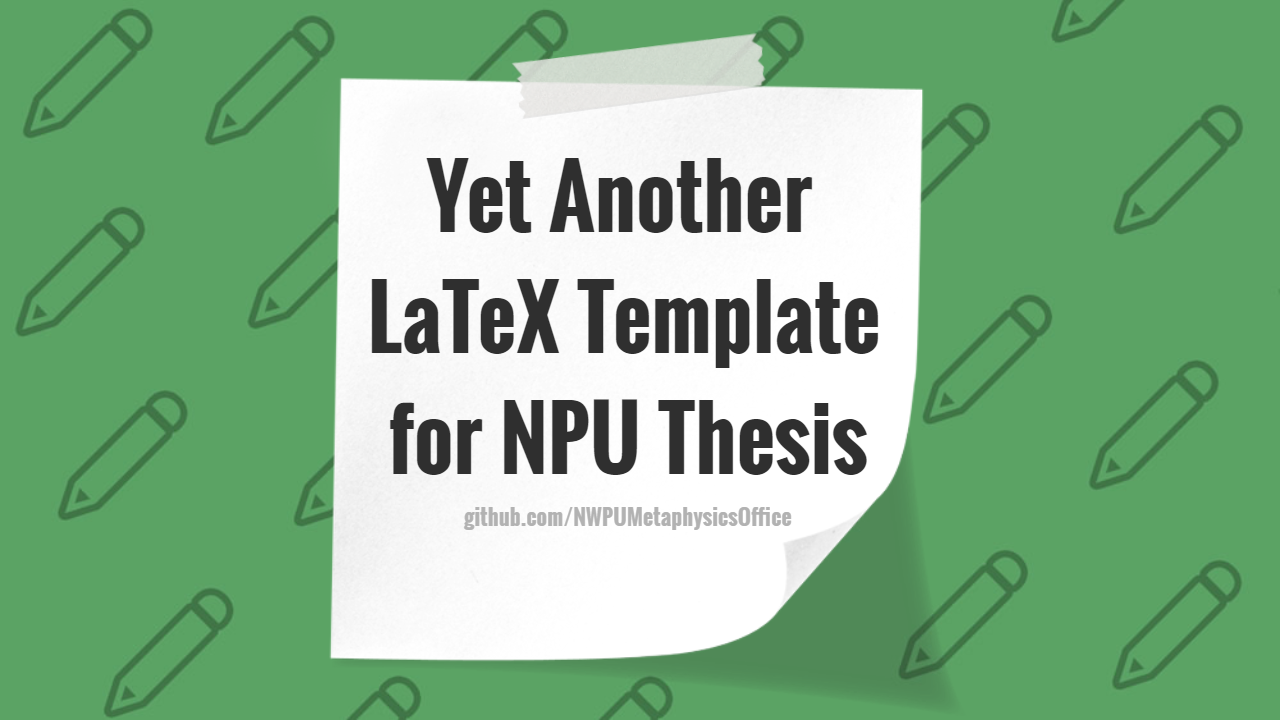
\includegraphics[scale=0.2]{poster.png}
    \caption{
        这里是个普通的标题
    }
    \label{fig:example}
\end{figure}

\begin{figure}[htb]
    \centering
    \begin{minipage}[t]{0.96\textwidth}
        \centering
        \begin{subfigure}[t]{0.47\textwidth}
            \centering
            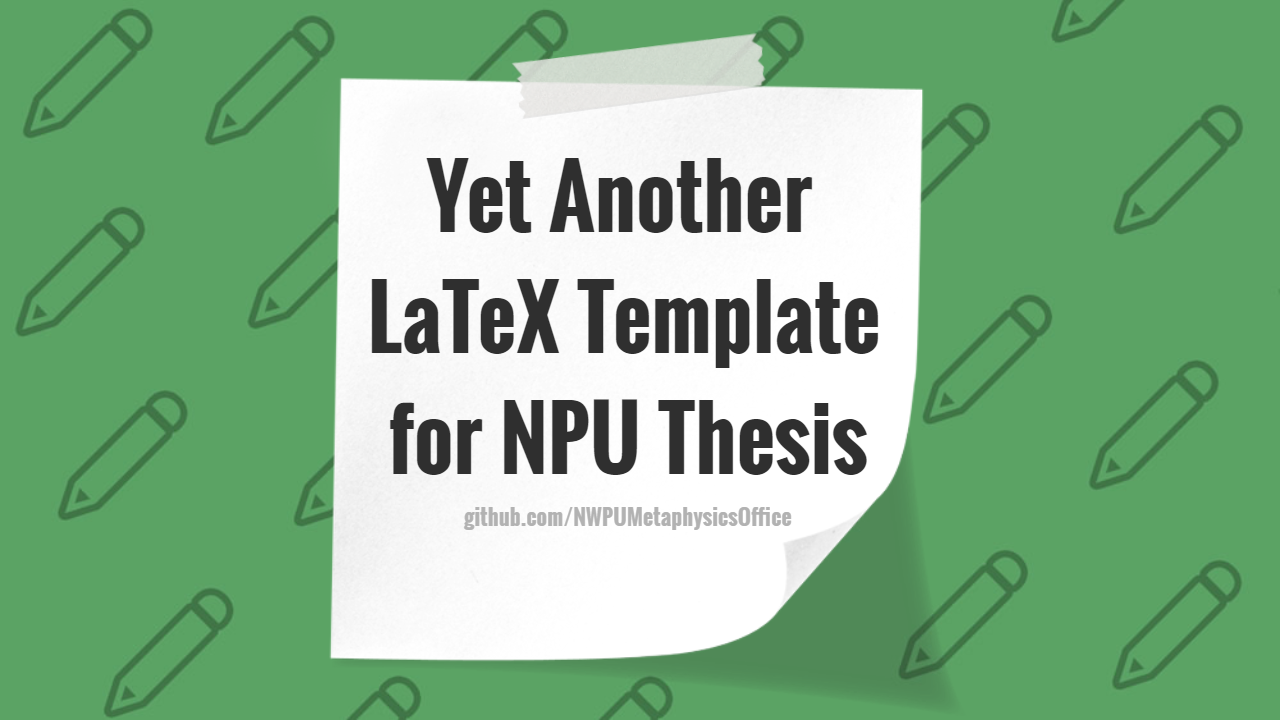
\includegraphics[scale=0.1]{poster.png}
            \caption{\label{subfig:example2-subfig1}}
        \end{subfigure}
        \begin{subfigure}[t]{0.47\textwidth}
            \centering
            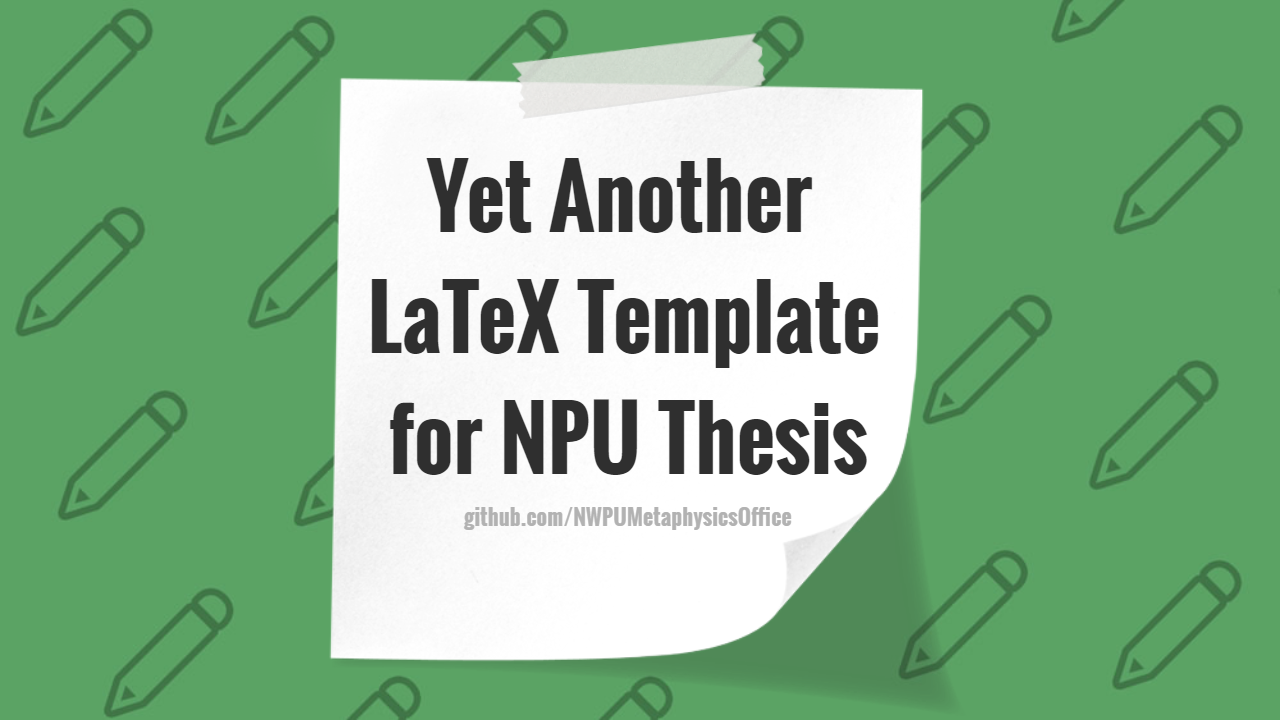
\includegraphics[scale=0.1]{poster.png}
            \caption{\label{subfig:example2-subfig2}}
        \end{subfigure}
    \end{minipage}
    \caption{这里是另一个普通的标题}
    \label{fig:example2}
\end{figure}

\section{插入源代码}

这里给出一个 Hello World 的样例,如\autoref{code:hello-world} 所示。

\begin{lstlisting}[language={C++}, label={code:hello-world},
    caption={Hello World.cpp}]
#include <iostream>
using namespace std;

int main()
{
    // output "Hello World!"
    cout << "Hello World!" << endl;
    return 0;
}
\end{lstlisting}

\section{引用以及其他编写建议}

\LaTeX 提供了 \lstinline`ref` 和 \lstinline`autoref` 两种引用方式,其中前者只显
示序号,后者可以显示提示语,如“\autoref{code:hello-world}”表示引用代码,
而“\autoref{subfig:example2-subfig2}”表示引用图片的子图.为了方便引用以及作者阅读,
本人强烈建议使用 \lstinline`autoref` 来统一处理引用问题,同时在每一个
\lstinline`autoref` 添加提示语,如 \lstinline`fig` 和 \lstinline`tab` 分别表示插
图和表格。

由于 \XeLaTeX 在处理中文时,会自动在中文之间添加空格,所以请放心地在编写文档时换
行,防止某一行过长导致阅读时的不便。另外中英文之间的空格(包括命令)并未做严格限
制。本文推荐除在不影响最终成文的结果这一前提下,为保持文档的美观与易读,请自行选
择合适的编写方式。

\cleardoublepage
%%=============================================================================%
%% 参考文献以及附录
%%-----------------------------------------------------------------------------%
\bibliographystyle{nputhesis}                               % 参考文献格式
\bibliography{reference}                                    % 参考文献
\appendix
\chapter{一份说明}

\section{测试附录子标题}

这是一份附录,请放置一些独立的证明、源代码、或其他辅助资料。

\nomenclature{$r$}{圆(或球)的半径}
\nomenclature{$C$}{圆的周长}
\nomenclature{$S$}{圆的面积}

\begin{equation}
    C = 2 \pi r
\end{equation}

\begin{equation}
    S = \pi r^2
\end{equation}

\cleardoublepage

\chapter{另一份说明}

这是另一份附录,请放置一些独立的证明、源代码、或其他辅助资料。

\nomenclature{$S_{\text{sphere}}$}{球的表面积}
\nomenclature{$V_{\text{sphere}}$}{球的体积}

\begin{equation}
    S_{\text{sphere}} = 4 \pi r^2
\end{equation}

\begin{equation}
    V_{\text{sphere}} = \frac43 \pi r^3
\end{equation}

\cleardoublepage
%%=============================================================================%
%% 文档附页部分(致谢、参加科研情况、知识产权与原创性声明)
%%-----------------------------------------------------------------------------%
\backmatter                                                 % 文档附页部分
%%-----------------------------------------------------------------------------%
\begin{acknowledgements}                                    % 致谢开始
    感谢我的老师和我的朋友们……
\end{acknowledgements}                                      % 致谢结束
%%-----------------------------------------------------------------------------%
\begin{accomplishments}                                     % 参加科研情况开始
    [1] ...
\end{accomplishments}                                       % 参加科研情况结束
%%-----------------------------------------------------------------------------%
\makestatement                                              % 知识产权与原创性声明
%%=============================================================================%
%% 文档结束
%%-----------------------------------------------------------------------------%
\end{document}
%%=============================================================================%


%%
%% This work consists of the file  yanputhesis.dtx
%% and the derived files           yanputhesis.ins,
%%                                 yanputhesis.pdf,
%%                                 yanputhesis.cls.
%%
%%
%% End of file `yanputhesis-sample.tex'.
